\documentclass[aspectratio=169]{beamer}

% ── Theme ────────────────────────────────────────────────────────────────────
\usetheme{Madrid}
\usecolortheme{seahorse}
\usefonttheme{professionalfonts}
\setbeamertemplate{navigation symbols}{}
\setbeamertemplate{footline}[frame number]
\setbeamerfont{frametitle}{size=\large,series=\bfseries}

% ── Packages ─────────────────────────────────────────────────────────────────
\usepackage{amsmath,amssymb}
\usepackage{booktabs}
\usepackage{colortbl}
\usepackage{xcolor}
\usepackage{tikz}
\usetikzlibrary{positioning}
\usepackage{fontspec}
\usepackage{graphicx}
\usepackage{array}
\usepackage{tabularx}
\usepackage{tcolorbox}
\tcbuselibrary{skins,breakable}

% ── Font ─────────────────────────────────────────────────────────────────────
\setmainfont{TeX Gyre Termes}
\setsansfont{TeX Gyre Heros}
\setmonofont{DejaVu Sans Mono}[Scale=0.85]

% ── Colours ──────────────────────────────────────────────────────────────────
\definecolor{primary}{RGB}{0,82,136}       % deep blue
\definecolor{accent}{RGB}{220,80,40}       % orange-red
\definecolor{good}{RGB}{30,140,60}         % green
\definecolor{bad}{RGB}{180,30,30}          % red
\definecolor{muted}{RGB}{100,100,110}      % grey
\definecolor{rowA}{RGB}{235,242,250}
\definecolor{rowB}{RGB}{255,255,255}
\definecolor{codebg}{RGB}{245,245,248}

\setbeamercolor{frametitle}{bg=primary,fg=white}
\setbeamercolor{title}{fg=primary}
\setbeamercolor{structure}{fg=primary}
\setbeamercolor{block title}{bg=primary!15,fg=primary}
\setbeamercolor{block body}{bg=primary!5}

% ── Custom boxes ─────────────────────────────────────────────────────────────
\newtcolorbox{keybox}[1][Key Takeaway]{
  colback=accent!8, colframe=accent, fonttitle=\bfseries\small,
  title=#1, left=4pt, right=4pt, top=3pt, bottom=3pt, sharp corners
}
\newtcolorbox{codebox}{
  colback=codebg, colframe=muted!40, fontupper=\ttfamily\small,
  left=6pt, right=6pt, top=4pt, bottom=4pt, sharp corners
}
\newtcolorbox{notebox}{
  colback=good!8, colframe=good!50, fontupper=\small\itshape,
  left=4pt, right=4pt, top=3pt, bottom=3pt, sharp corners
}

% ── Helpers ──────────────────────────────────────────────────────────────────
\newcommand{\yes}{\textcolor{good}{\textbf{Yes}}}
\newcommand{\no}{\textcolor{bad}{\textbf{No}}}
\newcommand{\highlight}[1]{\textcolor{accent}{\textbf{#1}}}
\newcommand{\code}[1]{\texttt{\small #1}}

% ── Meta ─────────────────────────────────────────────────────────────────────
\title[Span2Type]{\textbf{Span2Type}\\
  \large Improved Open-World Named Entity Recognition}
\subtitle{Motivation \& Problem Definition}
\author{Khoa Nguyen}
\date{April 27, 2026}

% ─────────────────────────────────────────────────────────────────────────────
\begin{document}

\begin{frame}
  \titlepage
\end{frame}

% ── Outline ──────────────────────────────────────────────────────────────────
\begin{frame}{Outline}
  \tableofcontents
\end{frame}

\section{Motivation}

% ── A1: Hook ─────────────────────────────────────────────────────────────────
\begin{frame}{Named Entity Recognition Powers Everything}
  \begin{columns}[T]
    \begin{column}{0.5\textwidth}
      \textbf{NER underpins:}
      \begin{itemize}\setlength\itemsep{6pt}
        \item Information extraction
        \item Knowledge graph construction
        \item Question answering
        \item Biomedical text mining
        \item Document understanding
      \end{itemize}
    \end{column}
    \begin{column}{0.5\textwidth}
      \begin{block}{State of the Art}
        BERT-based NER achieves\\[4pt]
        \centering\highlight{near-human performance}\\[4pt]
        on CoNLL-2003 \& OntoNotes
      \end{block}
      \vspace{10pt}
      \begin{keybox}[Open Question]
        If NER works so well on benchmarks ---\\
        \textbf{why can't we just deploy it everywhere?}
      \end{keybox}
    \end{column}
  \end{columns}
\end{frame}

% ── A2: Closed-World Assumption ───────────────────────────────────────────────
\begin{frame}{The Hidden Assumption Breaking Real-World NER}
  \begin{center}
  \renewcommand{\arraystretch}{1.4}
  \begin{tabular}{>{\bfseries\color{primary}}p{4.2cm}|p{4.8cm}}
    \toprule
    \rowcolor{primary!15}
    \textcolor{primary}{\textbf{Benchmark Setting}} &
    \textcolor{accent}{\textbf{Real World}} \\
    \midrule
    \rowcolor{rowA}
    Types fixed in advance & Types \highlight{unknown}, evolve over time \\
    \rowcolor{rowB}
    Large labeled training set & Annotation: expensive, slow, expert-needed \\
    \rowcolor{rowA}
    One domain, one ontology & New domains emerge constantly \\
    \rowcolor{rowB}
    \code{ORG / PER / LOC / MISC} &
      \code{Protein / Subsystem / Regulatory Mechanism} \\
    \bottomrule
  \end{tabular}
  \end{center}
  \vspace{8pt}
  \begin{keybox}[Closed-World Assumption]
    Every high-performing NER system assumes the type set is
    \textbf{predefined} and \textbf{labeled examples exist} for each type.
    This is convenient for benchmarks --- but a
    \highlight{fundamental deployment barrier}.
  \end{keybox}
\end{frame}

\section{Five Challenges}

% ── Challenge overview (mini-roadmap) ────────────────────────────────────────
\begin{frame}{Five Open Problems in Open-World NER}
  \begin{center}
  \renewcommand{\arraystretch}{1.5}
  \begin{tabular}{>{\bfseries\color{primary}}c p{9.5cm}}
    C1 & Span boundaries break under domain shift \\
    \hline
    C2 & The type inventory is unknown \\
    \hline
    C3 & Cluster IDs are not interpretable \\
    \hline
    C4 & Full fine-tuning is too expensive per domain \\
    \hline
    C5 & Standard metrics fail for open-vocabulary names \\
  \end{tabular}
  \end{center}
  \vspace{6pt}
  \begin{notebox}
    Each challenge motivates one targeted design decision in Span2Type.
  \end{notebox}
\end{frame}

% ── A3: Challenge 1 ───────────────────────────────────────────────────────────
\begin{frame}{C1 --- Span Boundaries Break Under Domain Shift}

  \begin{columns}[T]
    \begin{column}{0.50\textwidth}
      \begin{codebox}
        \textcolor{good}{\textbf{Source} (newswire):}\\[3pt]
        ``\underline{Germany} defeated \underline{Brazil} 2-1.''\\
        \textcolor{good}{\small $\checkmark$\ Simple nouns — BIO handles fine}\\[10pt]
        \textcolor{bad}{\textbf{Target} (CrossNER-AI):}\\[3pt]
        ``We apply \textbf{support vector machine}\\
        \phantom{``We apply }to image classification.''\\
        \textcolor{bad}{\small $\times$\ 3-token span — BIO often splits it}
      \end{codebox}
    \end{column}
    \begin{column}{0.46\textwidth}
      \textbf{Root cause:} BIO sees \highlight{one signal} only\\[6pt]
      \begin{tabular}{cl}
        \textbf{BIO} & sequential per-token tags \\[4pt]
        \textbf{SE}  & start / end boundary tokens \\[4pt]
        \textbf{TB}  & adjacent token co-membership \\
      \end{tabular}
      \vspace{10pt}
      \begin{keybox}
        All three views exist.\\
        OWNER uses only BIO.\\[4pt]
        \highlight{60.5 F1} on CrossNER-AI\\
        — lowest of all 5 domains.
      \end{keybox}
    \end{column}
  \end{columns}
\end{frame}

% ── A4: Challenge 2 ───────────────────────────────────────────────────────────
\begin{frame}{C2 --- The Type Inventory Is Unknown}

  \begin{center}
  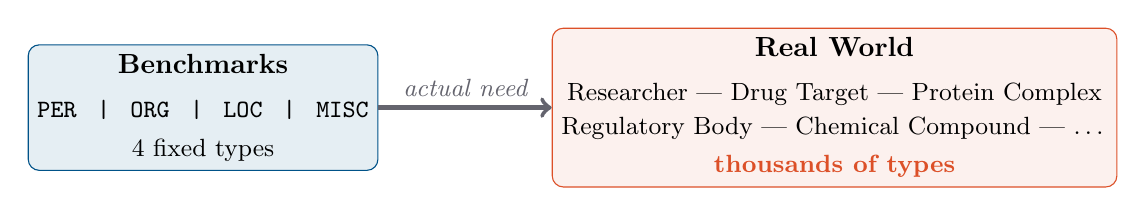
\begin{tikzpicture}
    \node[draw=primary,fill=primary!10,rounded corners,
          minimum width=3.6cm,minimum height=1.4cm,align=center]
      (A) {\textbf{Benchmarks}\\[4pt]
           \small\code{PER \;|\; ORG \;|\; LOC \;|\; MISC}\\[2pt]
           \small 4 fixed types};
    \node[draw=accent,fill=accent!8,rounded corners,
          minimum width=5.8cm,minimum height=1.4cm,align=center,
          right=2.2cm of A]
      (B) {\textbf{Real World}\\[4pt]
           \small Researcher\ |\ Drug Target\ |\ Protein Complex\\
           \small Regulatory Body\ |\ Chemical Compound\ |\ \ldots\\[2pt]
           \textcolor{accent}{\small\bfseries thousands of types}};
    \draw[->,ultra thick,color=muted] (A.east) -- (B.west)
      node[midway,above,font=\small\itshape,color=muted] {actual need};
  \end{tikzpicture}
  \end{center}

  \vspace{6pt}
  \begin{columns}[T]
    \begin{column}{0.50\textwidth}
      \begin{itemize}\setlength\itemsep{5pt}
        \item Real-world types number in the \textbf{thousands}
              \small{(Choi et al., 2018)}
        \item Supervised NER only classifies \emph{trained} types
        \item New types are invisible to closed-world systems
      \end{itemize}
    \end{column}
    \begin{column}{0.46\textwidth}
      \begin{keybox}[GLiNER / UniversalNER still fail here]
        \small``Zero-shot'' NER still requires a human to
        \highlight{supply type names at inference}.\\[4pt]
        True open-world: the system \textbf{discovers types by itself}.
      \end{keybox}
    \end{column}
  \end{columns}
\end{frame}

% ── A5: Challenge 3 ───────────────────────────────────────────────────────────
\begin{frame}{C3 --- Cluster IDs Are Not Entity Types}

  \begin{columns}[T]
    \begin{column}{0.46\textwidth}
      \textbf{\textcolor{bad}{Prior work stops here:}}
      \vspace{5pt}
      \begin{codebox}
        ``Albert Einstein'' $\;\to\;$ \textbf{Cluster 3}\\
        ``Marie Curie''\ \ \ \ $\;\to\;$ \textbf{Cluster 3}\\
        ``Watson''\ \ \ \ \ \ \ \ \ $\;\to\;$ \textbf{Cluster 7}\\[8pt]
        \textcolor{bad}{What is Cluster 3?}\\
        \textcolor{bad}{Cannot validate. Cannot deploy.}
      \end{codebox}
    \end{column}
    \begin{column}{0.50\textwidth}
      \textbf{\textcolor{good}{Span2Type goes further:}}
      \vspace{5pt}
      \begin{codebox}
        Cluster 3 $\;\to\;$ \textcolor{good}{\textbf{``Physicist''}}\\
        Cluster 7 $\;\to\;$ \textcolor{good}{\textbf{``Fictional Character''}}\\[8pt]
        \textcolor{good}{$\checkmark$\ Expert-validatable}\\
        \textcolor{good}{$\checkmark$\ Knowledge-base ready}\\
        \textcolor{good}{$\checkmark$\ Downstream-usable}
      \end{codebox}
    \end{column}
  \end{columns}
  \vspace{8pt}
  \begin{keybox}
    Naming is \highlight{not cosmetic} ---
    it is what makes unsupervised clusters \textbf{actionable}.
  \end{keybox}
\end{frame}

% ── A6: Challenge 4 ───────────────────────────────────────────────────────────
\begin{frame}{C4 --- Full Fine-Tuning Is Too Expensive per Domain}

  \begin{center}
  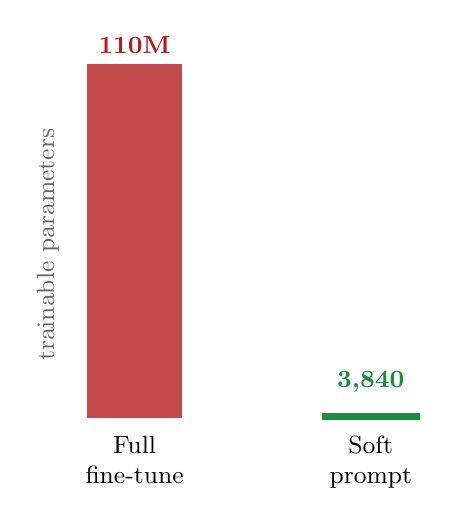
\begin{tikzpicture}
    % Left bar
    \fill[bad!80] (0,0) rectangle (1.2,4.5);
    \node[above,font=\small\bfseries,color=bad] at (0.6,4.5) {110M};
    \node[below,font=\small,align=center] at (0.6,-0.1)
      {Full\\fine-tune};
    % Right bar
    \fill[good!70] (3.0,0) rectangle (4.2,0.04);
    \draw[good,very thick] (3.0,0) rectangle (4.2,0.04);
    \node[above,font=\small\bfseries,color=good] at (3.6,0.2) {3,840};
    \node[below,font=\small,align=center] at (3.6,-0.1)
      {Soft\\prompt};
    % y-label
    \node[rotate=90,font=\small,color=muted] at (-0.5,2.2)
      {trainable parameters};
  \end{tikzpicture}
  \end{center}

  \begin{columns}[T]
    \begin{column}{0.50\textwidth}
      \textbf{\textcolor{bad}{Full fine-tuning risks:}}
      \begin{itemize}\setlength\itemsep{3pt}
        \item Costly per new domain
        \item Catastrophic forgetting of pre-trained weights
      \end{itemize}
    \end{column}
    \begin{column}{0.46\textwidth}
      \begin{keybox}[Solution: two-stage schedule]
        \small Stage 1: backbone \textbf{frozen}, prompt warms up\\
        Stage 2: backbone unlocked at $100\times$ lower LR\\
        Optimizer moments \textbf{preserved} across boundary
      \end{keybox}
    \end{column}
  \end{columns}
\end{frame}

% ── A7: Challenge 5 ───────────────────────────────────────────────────────────
\begin{frame}{C5 --- Standard Metrics Fail for Open-Vocabulary Names}

  \begin{columns}[T]
    \begin{column}{0.46\textwidth}
      \textbf{\textcolor{bad}{Exact match is misleading:}}
      \vspace{5pt}
      \begin{codebox}
        Gold:\ \ \ \ \code{"musicalartist"}\\
        Output:\ \ \code{"musician"}\\
        \textcolor{bad}{Exact-match score: 0}\\
        \textcolor{good}{Semantic reality: correct}\\[8pt]
        Gold:\ \ \ \ \code{"researcher"}\\
        Output:\ \ \code{"physicist"}\\
        \textcolor{bad}{Exact-match score: 0}\\
        \textcolor{good}{Semantic reality: close hyponym}
      \end{codebox}
    \end{column}
    \begin{column}{0.50\textwidth}
      \textbf{BERTScore-F1 calibration:}
      \vspace{5pt}
      \begin{tabular}{lc}
        \toprule
        Prediction quality & Score \\
        \midrule
        Exact copy         & 1.00 \\
        Synonym / hyponym  & $\approx 0.95$ \\
        Related but off    & $\approx 0.90$ \\
        Completely wrong   & $\approx 0.86$ \\
        \bottomrule
      \end{tabular}
      \vspace{8pt}
      \begin{keybox}
        Signal lives in $[0.86,\;1.0]$.\\
        Reproducible \& scalable ---\\
        human eval infeasible at this scale.
      \end{keybox}
    \end{column}
  \end{columns}
\end{frame}

% ── A8: Summary roadmap ──────────────────────────────────────────────────────
\begin{frame}{Challenges $\to$ Contributions}
  \begin{center}
  \renewcommand{\arraystretch}{1.5}
  \begin{tabular}{>{\bfseries\color{primary}}c p{4.8cm} p{5.2cm}}
    \toprule
    \rowcolor{primary!15}
    & \textbf{Challenge} & \textbf{Our Answer} \\
    \midrule
    \rowcolor{rowA}
    C1 & Brittle single-view span detection
       & DTrans: BIO $+$ SE $+$ TB union \\
    \rowcolor{rowB}
    C2 & Unknown type inventory
       & BIC-guided auto $k^*$ selection \\
    \rowcolor{rowA}
    C3 & Cluster IDs not interpretable
       & MMR exemplar selection $+$ LLM naming \\
    \rowcolor{rowB}
    C4 & Fine-tuning cost per domain
       & Two-stage soft prompt (3,840 params) \\
    \rowcolor{rowA}
    C5 & No metric for open-vocab names
       & BERTScore-F1 as semantic proxy \\
    \bottomrule
  \end{tabular}
  \end{center}
  \vspace{4pt}
  \begin{notebox}
    Every methodology design choice traces back to a row in this table.
  \end{notebox}
\end{frame}

\section{Problem Definition}

% ── B1: Formal definition ────────────────────────────────────────────────────
\begin{frame}{Formal Problem Statement}
  \begin{block}{Input}
    An \textbf{unannotated} target-domain corpus $\mathcal{D}_T$\\
    No gold entity spans \;|\; no type labels \;|\; no ontology
  \end{block}
  \vspace{6pt}
  \begin{block}{Goal --- Three Outputs}
    \begin{enumerate}\setlength\itemsep{5pt}
      \item \textbf{Span detection:} identify all entity mention spans in $\mathcal{D}_T$
      \item \textbf{Entity typing:} group spans into coherent semantic clusters
        (unsupervised, $k$ \emph{unknown})
      \item \textbf{Cluster naming:} assign a concise, human-readable label
        to each cluster
    \end{enumerate}
  \end{block}
  \vspace{6pt}
  \begin{keybox}[Evaluation constraint]
    Gold CrossNER labels used \textbf{strictly for evaluation} ---
    never seen during training, clustering, or naming.
  \end{keybox}
\end{frame}

% ── B2: Open-world vs closed-world ──────────────────────────────────────────
\begin{frame}{Open-World vs.\ Closed-World NER}
  \begin{center}
  \renewcommand{\arraystretch}{1.4}
  \begin{tabular}{p{3.2cm}|>{\centering\arraybackslash}p{3.2cm}|>{\centering\arraybackslash}p{3.6cm}}
    \toprule
    \rowcolor{primary!15}
    \textbf{Property}
      & \textbf{Closed-World NER}
      & \textbf{Open-World (Span2Type)} \\
    \midrule
    \rowcolor{rowA}
    Type set at train time & Fixed, known & \highlight{Unknown} \\
    \rowcolor{rowB}
    Labeled target data & Required & \textcolor{good}{Not used} \\
    \rowcolor{rowA}
    Output & Span + predefined type
            & Span + discovered type + \textbf{name} \\
    \rowcolor{rowB}
    Handles new types? & \no & \yes \\
    \rowcolor{rowA}
    Example types & \code{PER, ORG, LOC}
                  & \code{Physicist, Drug Compound} \\
    \bottomrule
  \end{tabular}
  \end{center}
\end{frame}

% ── B3: Evaluation setup ─────────────────────────────────────────────────────
\begin{frame}{How We Measure Success}
  \begin{center}
  \renewcommand{\arraystretch}{1.4}
  \begin{tabular}{p{2.8cm}|p{3.2cm}|p{5.2cm}}
    \toprule
    \rowcolor{primary!15}
    \textbf{Stage} & \textbf{Metric} & \textbf{What It Measures} \\
    \midrule
    \rowcolor{rowA}
    Entity Detection
      & Span F1 (exact)
      & Precision / Recall of span boundaries \\
    \rowcolor{rowB}
    Entity Typing
      & AMI
      & Cluster quality vs.\ gold partition --- no label mapping needed \\
    \rowcolor{rowA}
    Cluster Naming
      & BERTScore-F1
      & Semantic similarity: predicted vs.\ gold type name \\
    \bottomrule
  \end{tabular}
  \end{center}
  \vspace{8pt}
  \begin{columns}[T]
    \begin{column}{0.48\textwidth}
      \begin{block}{Source}
        \textbf{CoNLL-2003} (4 types, newswire)\\
        \small Detector training only
      \end{block}
    \end{column}
    \begin{column}{0.48\textwidth}
      \begin{block}{Target}
        \textbf{CrossNER} --- 5 domains\\
        \small AI \;|\; Literature \;|\; Music \;|\; Politics \;|\; Science\\
        \small 9--17 gold types each
      \end{block}
    \end{column}
  \end{columns}
\end{frame}

% ── End ──────────────────────────────────────────────────────────────────────
\begin{frame}[plain]
  \begin{center}
    {\Large\bfseries\color{primary} End of Section}\\[12pt]
    {\large Motivation \& Problem Definition}\\[20pt]
    \textcolor{muted}{\small Next: Methodology --- Three Contributions}
  \end{center}
\end{frame}

\end{document}
